<<<<<<< HEAD
\documentclass[10pt]{beamer}
\usepackage{style_presentation} %See style_presentation.sty for detailed packages
\addbibresource{references_presentation.bib}
=======
 \documentclass[10pt]{beamer}
 \usepackage{style_presentation} %See style_presentation.sty for detailed packages

%put this all into mybib because its ugly
\usetheme{Madrid}
\definecolor{teall}{RGB}{5, 77, 79}
\definecolor{strategyblue}{RGB}{51, 102, 153}
\definecolor{datagreen}{RGB}{34, 139, 34}
\definecolor{boxbg}{RGB}{245, 245, 245} % Light gray for box background
\usecolortheme[named=teall]{structure}
>>>>>>> 1a19774ded2f08b42fe103161d958e218e36807a

%footnote
\setbeamertemplate{navigation symbols}{}
\setbeamertemplate{footline}{}
\setbeamertemplate{footline}{%
  \hfill%
  \usebeamerfont{page number in head/foot}%
  \usebeamercolor[fg]{page number in head/foot}%
  \insertframenumber\,/\,\inserttotalframenumber%
  \hspace*{2ex}%
}
\setbeamercolor{page number in head/foot}{fg=black}


%Titlepage
\title{Swiss Performance Index Momentum Strategy}
\subtitle{Project Paper: Digital Tools for Finance}
\author{Iris Bodenmann, Justin Meichtry, Maurice Kammermann, Steve Nikitas}
\titlegraphic{
\includegraphics[height=1.5cm]{Universität_Zürich_logo.png}}
\date{11th of December 2024}
\institute[]{Igor Pozdeev\\Department of Finance\\ University of Zurich}

\begin{document}
\begin{frame}
\maketitle
\end{frame}

%Table of Contents
\begin{frame}
\frametitle{Table of Contents}
\tableofcontents
\end{frame}

%Introduction
\section{Introduction}
\begin{frame}{Introduction}
\begin{itemize}
    \item Momentum ranks among the most pervasive stock market anomalies, serving as a cornerstone for extensive research and investment strategies.
<<<<<<< HEAD
    \item Our project investigates the efficacy of long-only momentum strategies, as introduced by \cite{jegatit1993}, in delivering excess returns within the Swiss stock market over the period from 2000 to 2024.
=======
    \item Our project investigates the efficacy of long-only momentum strategies, as introduced by Jegadeesh and Titman (1993), in delivering excess returns within the Swiss stock market over the period from 2000 to 2024.
>>>>>>> 1a19774ded2f08b42fe103161d958e218e36807a
    \item By focusing on the Swiss market, this study sheds light on momentum effects in a smaller, less-researched and less liquid market, contributing to the understanding of anomaly persistence across different contexts.
    \item The findings aim to bridge the gap between academic theory and practical application, offering insights for investors in designing robust market strategies.
\end{itemize}
\end{frame}



% Data and Methodology
\section{Data and Methodology}
<<<<<<< HEAD
\begin{frame}[fragile]{Data and Methodology}
=======
\begin{frame}[fragile]{Methodology}
>>>>>>> 1a19774ded2f08b42fe103161d958e218e36807a

\noindent % Ensure no indentation
\begin{minipage}[t]{0.45\textwidth} % Left box
    \begin{tcolorbox}[colframe=datagreen, colback=boxbg, coltitle=white, title=Data, sharp corners=all, fonttitle=\bfseries, left=2mm, right=2mm, enhanced, height=6cm]
        Swiss stock market was proxied using the SPI. 
        \begin{itemize}
            \item \textbf{Benchmark:} SPI Total Return Index. Daily data from Refinitiv.
            \item \textbf{Risk-Free:} 1-year Swiss government bond yield. Monthly data from SNB API.
            \item \textbf{Time Period:} January 2000 - November 2024
        \end{itemize}
    \end{tcolorbox}
\end{minipage}%
\hspace{0.05\textwidth} % Horizontal spacing
\begin{minipage}[t]{0.45\textwidth} % Right box
    \begin{tcolorbox}[colframe=strategyblue, colback=boxbg, coltitle=white, title=Methodology, sharp corners=all, fonttitle=\bfseries, left=2mm, right=2mm, enhanced, height=6cm]
        \begin{itemize}
            \item \textbf{Holding Period:} 6 months
            \item \textbf{Lookback Period:} 6 months
            \item \textbf{Weighting:} Equally weighted
            \item \textbf{Rebalancing:} Monthly
            \item \textbf{Transaction costs:} Proportional, up to 1\%
            
        \end{itemize}
    \end{tcolorbox}
\end{minipage}

\end{frame}

% Results
<<<<<<< HEAD
\section{Results}
\begin{frame}{Results: Long Only and Long/Short Momentum vs. SPI}
   \begin{figure}
   \caption{Cumulative Total Returns: Long Only and Long/Short Momentum vs. SPI}
        \centering
        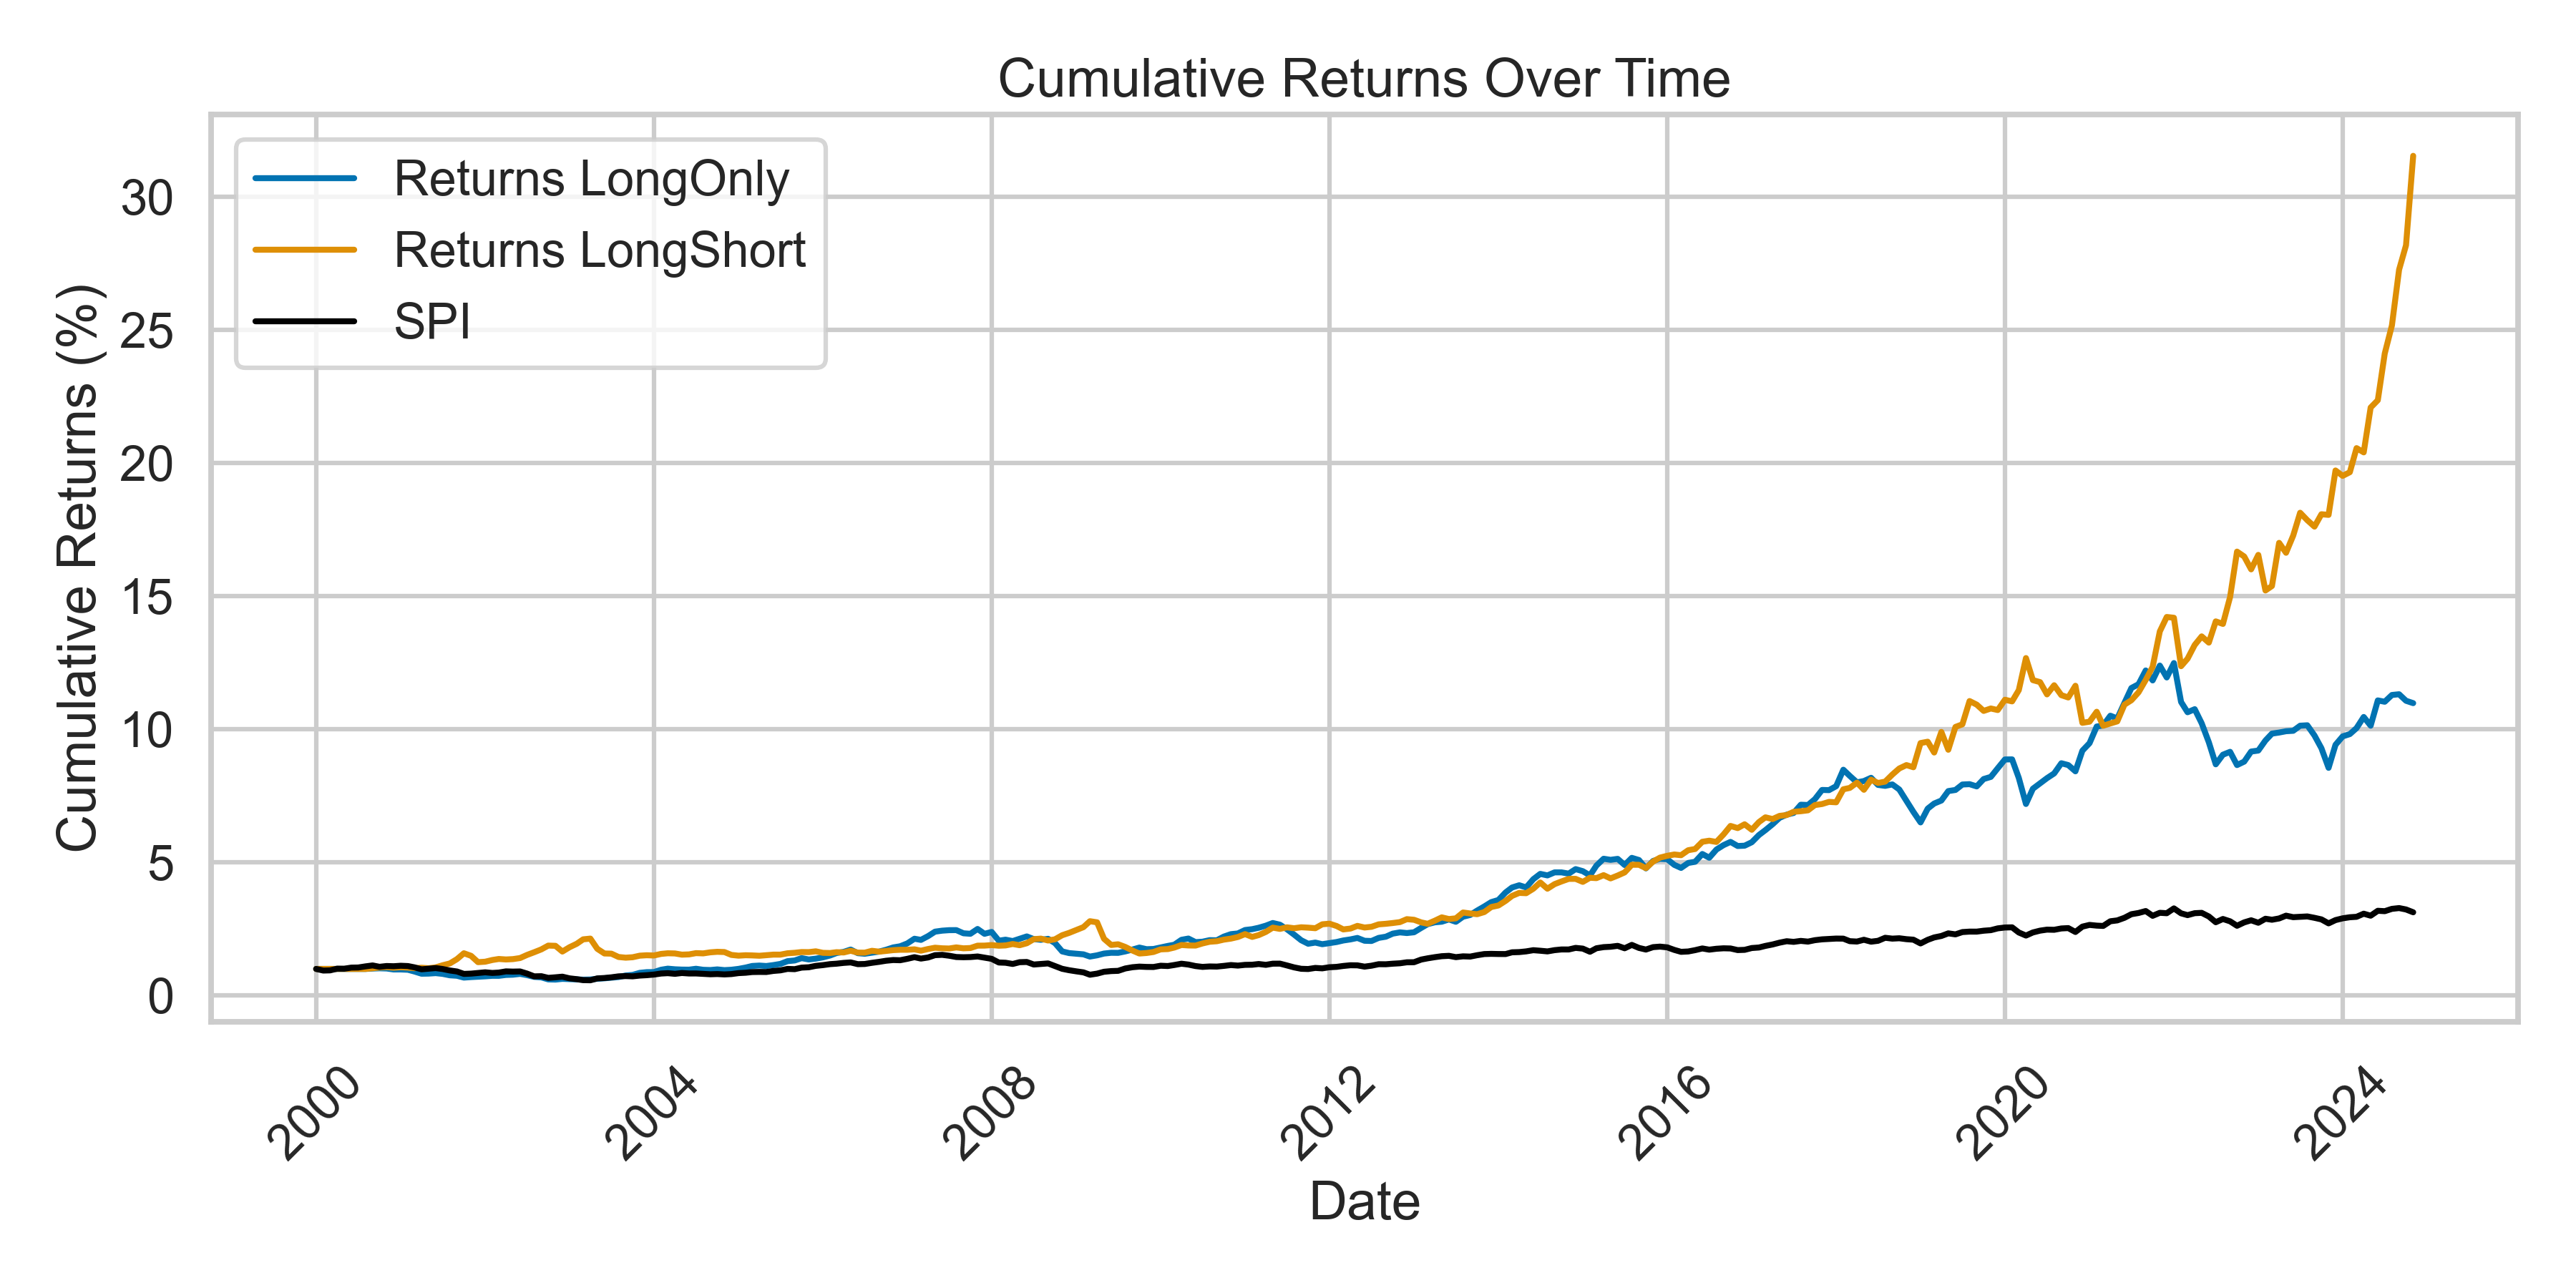
\includegraphics[width=\linewidth]{figures/cumulative_returns.png}
    \end{figure}
\end{frame}

\begin{frame}{Summary Statistics: Long Only and Long/Short Momentum vs. SPI}
\begin{table}
\centering
\resizebox{\textwidth}{!}{
\begin{tabular}{l S[table-format=2.4] S[table-format=2.4] S[table-format=1.4]}

\toprule
\multirow{2}{*}{Metric} & \multicolumn{3}{c}{Strategies} \\
\cmidrule(l){2-4}
& {Long-Only} & {Long/Short} & {Benchmark} \\
\midrule
Avg Total Return (Geometric) & 10.0953 & 18.7608 & 1.4619 \\
Avg Excess Return (Geometric) & 8.2598 & 16.9252 & -0.4619 \\
Std Dev of Excess Returns & 0.0438 & 0.0530 & 0.0401 \\
Std of Excess Returns (Annualized) & 0.1517 & 0.1835 & 0.1388 \\
Sharpe Ratio (Geometric) & 0.5443 & 0.9225 & -0.0333 \\
Min Excess Return & -0.1627 & -0.2214 & -0.1302 \\
Max Excess Return & 0.0990 & 0.1452 & 0.1202 \\
Skewness of Excess Return & -0.7074 & -0.5370 & -0.4670 \\
Kurtosis of Excess Return & 0.9103 & 2.6598 & 0.1039 \\
Alpha (Geometric) & 5.9176 & 18.6500 & 0.0000 \\
T-stat of Alpha & 3.0654 & 5.3641 & -109.7906 \\
Beta (Factor Return) & 0.8642 & -0.4478 & 1.0000 \\
\bottomrule
\end{tabular}
}
\caption{Summary Statistics Long-Only and Long/Short vs. Benchmark}
\end{table}


=======
\begin{frame}{Results}
    \begin{center}
        {\footnotesize \textbf{Cumulative Returns: Net-Cumulative Total Returns Long Only Momentum vs. SPI}}
        \vspace{0.5cm} % Adjust spacing as needed
        \includegraphics[width=\linewidth]{rc_trxCost.png}
    \end{center}
>>>>>>> 1a19774ded2f08b42fe103161d958e218e36807a
\end{frame}


%Robustness Check
\section{Robustness Check}
\begin{frame}{Robustness Check}

We explored the variability of various parameters that may impact performance and cost-effectiveness:

\begin{itemize}
    \item Holding period
    \item Lookback period
    \item Number of assets held
    \item Transaction costs    
\end{itemize}
\end{frame}

<<<<<<< HEAD
\begin{frame}{Robustness Check: Varying Holding Period Months}
  \begin{figure}
   \caption{Sharpe Ratios Over Different Holding Period Months}
        \centering
        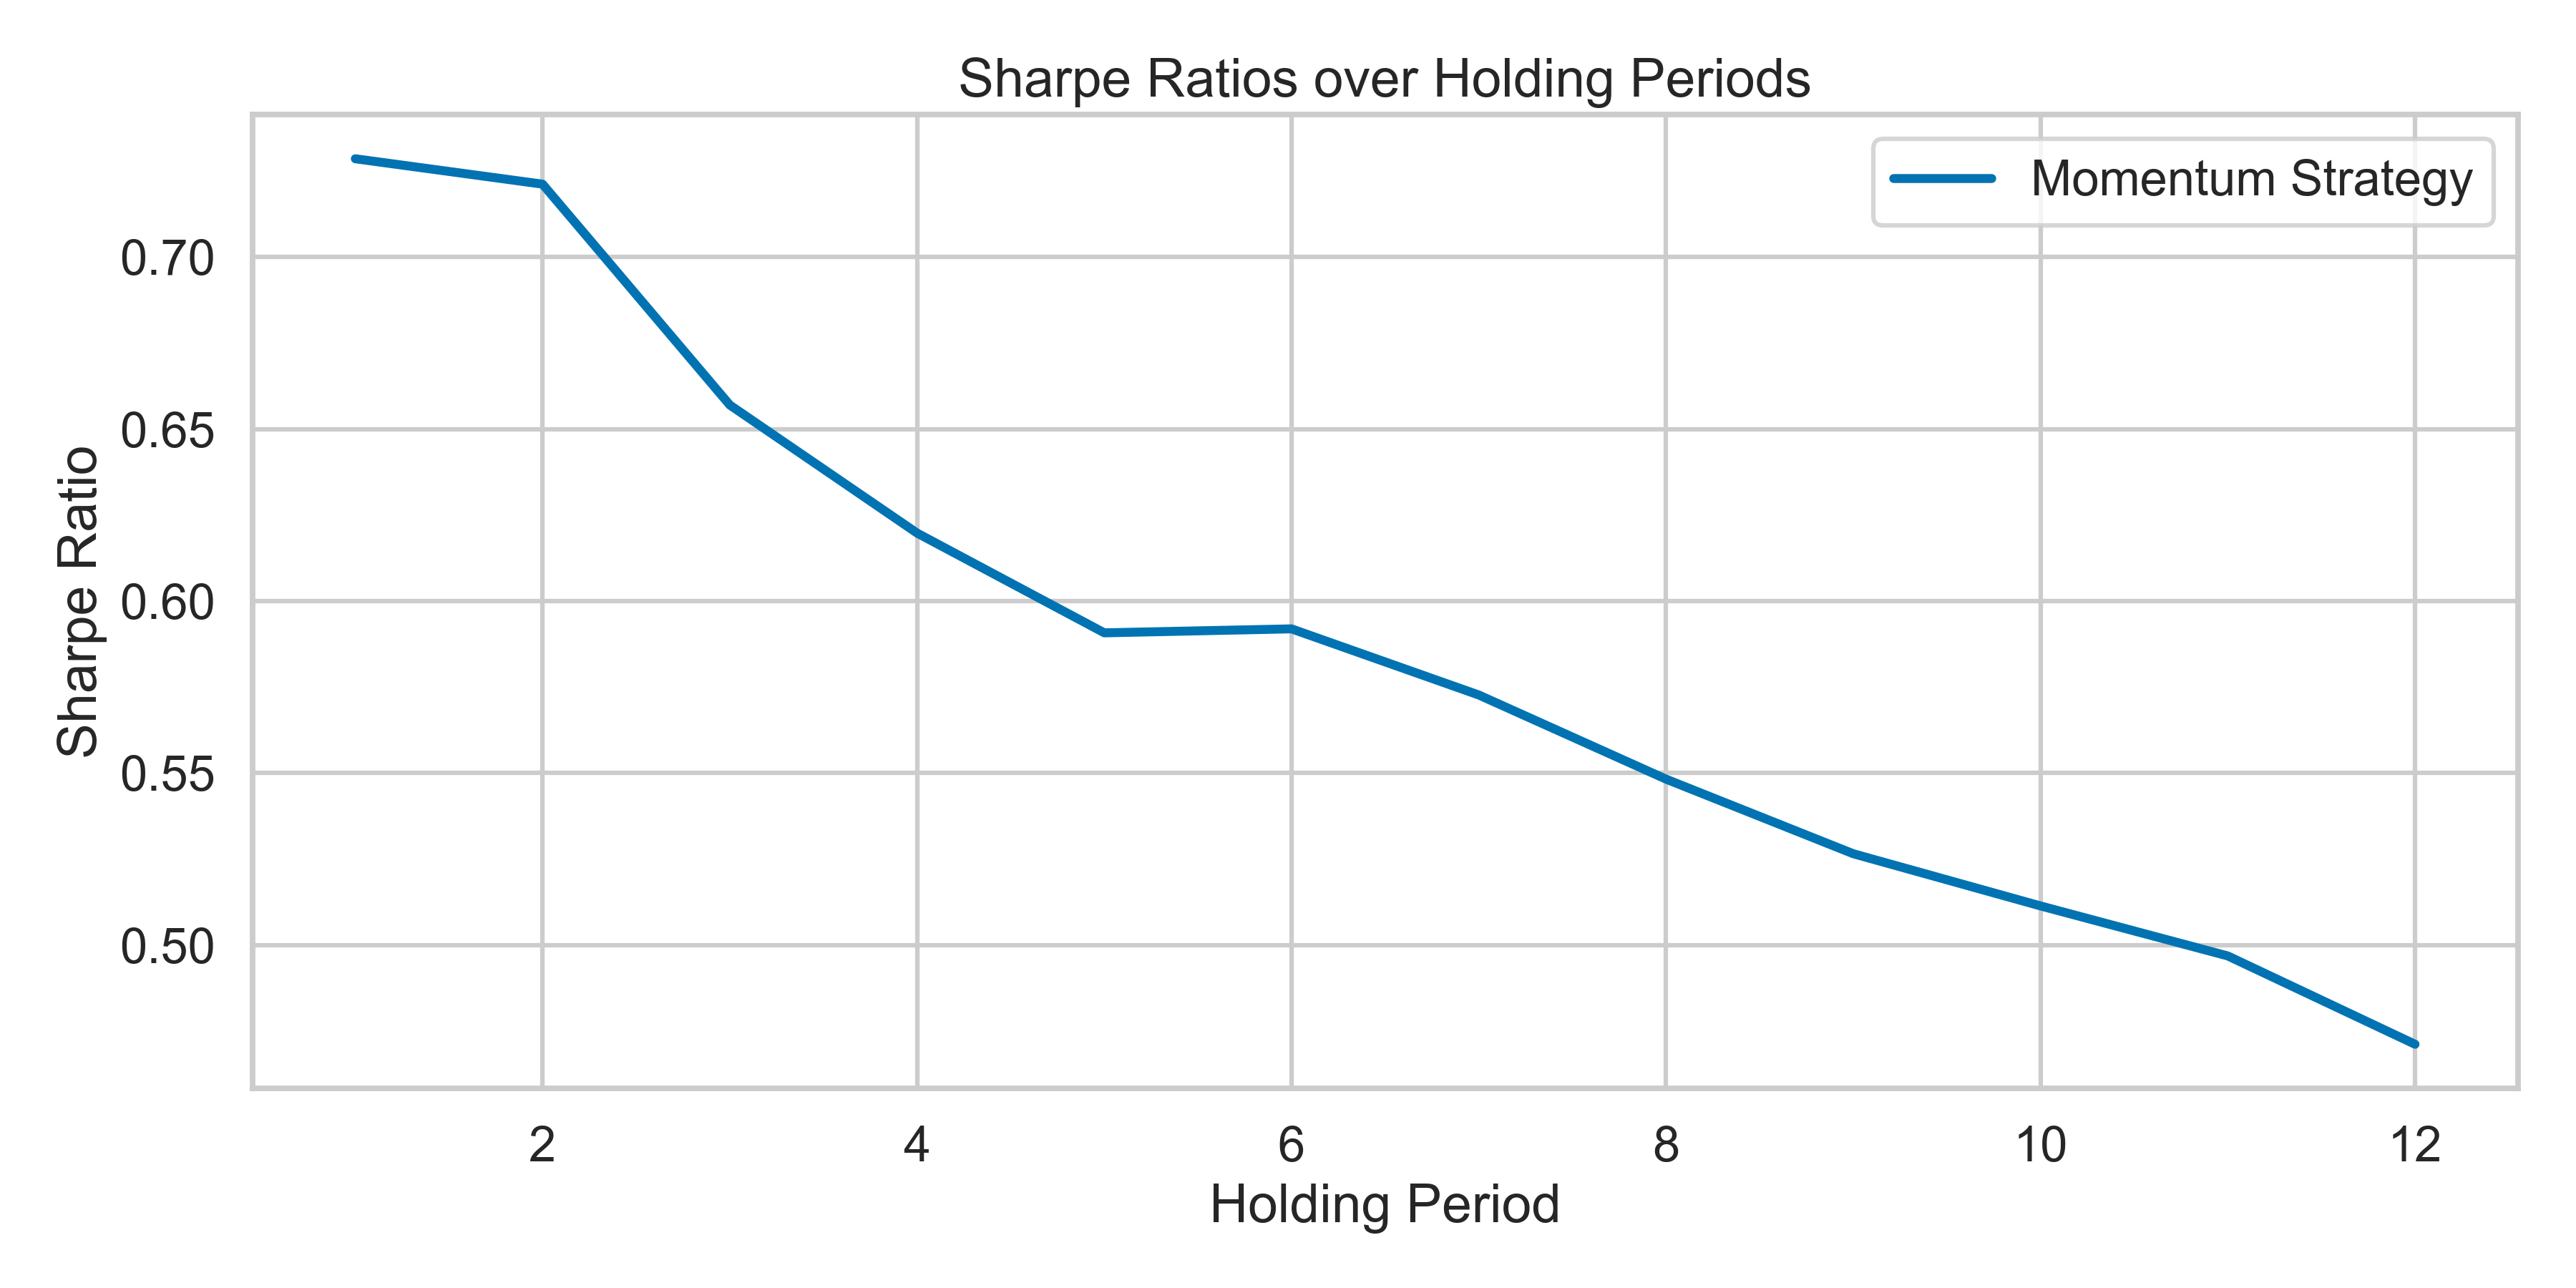
\includegraphics[width=\linewidth]{figures/rc_holding_period.png}
    \end{figure}
\end{frame}

\begin{frame}{Robustness Check: Varying Lookback Period Months}
  \begin{figure}
   \caption{Sharpe Ratios Over Different Lookback Period Months}
        \centering
        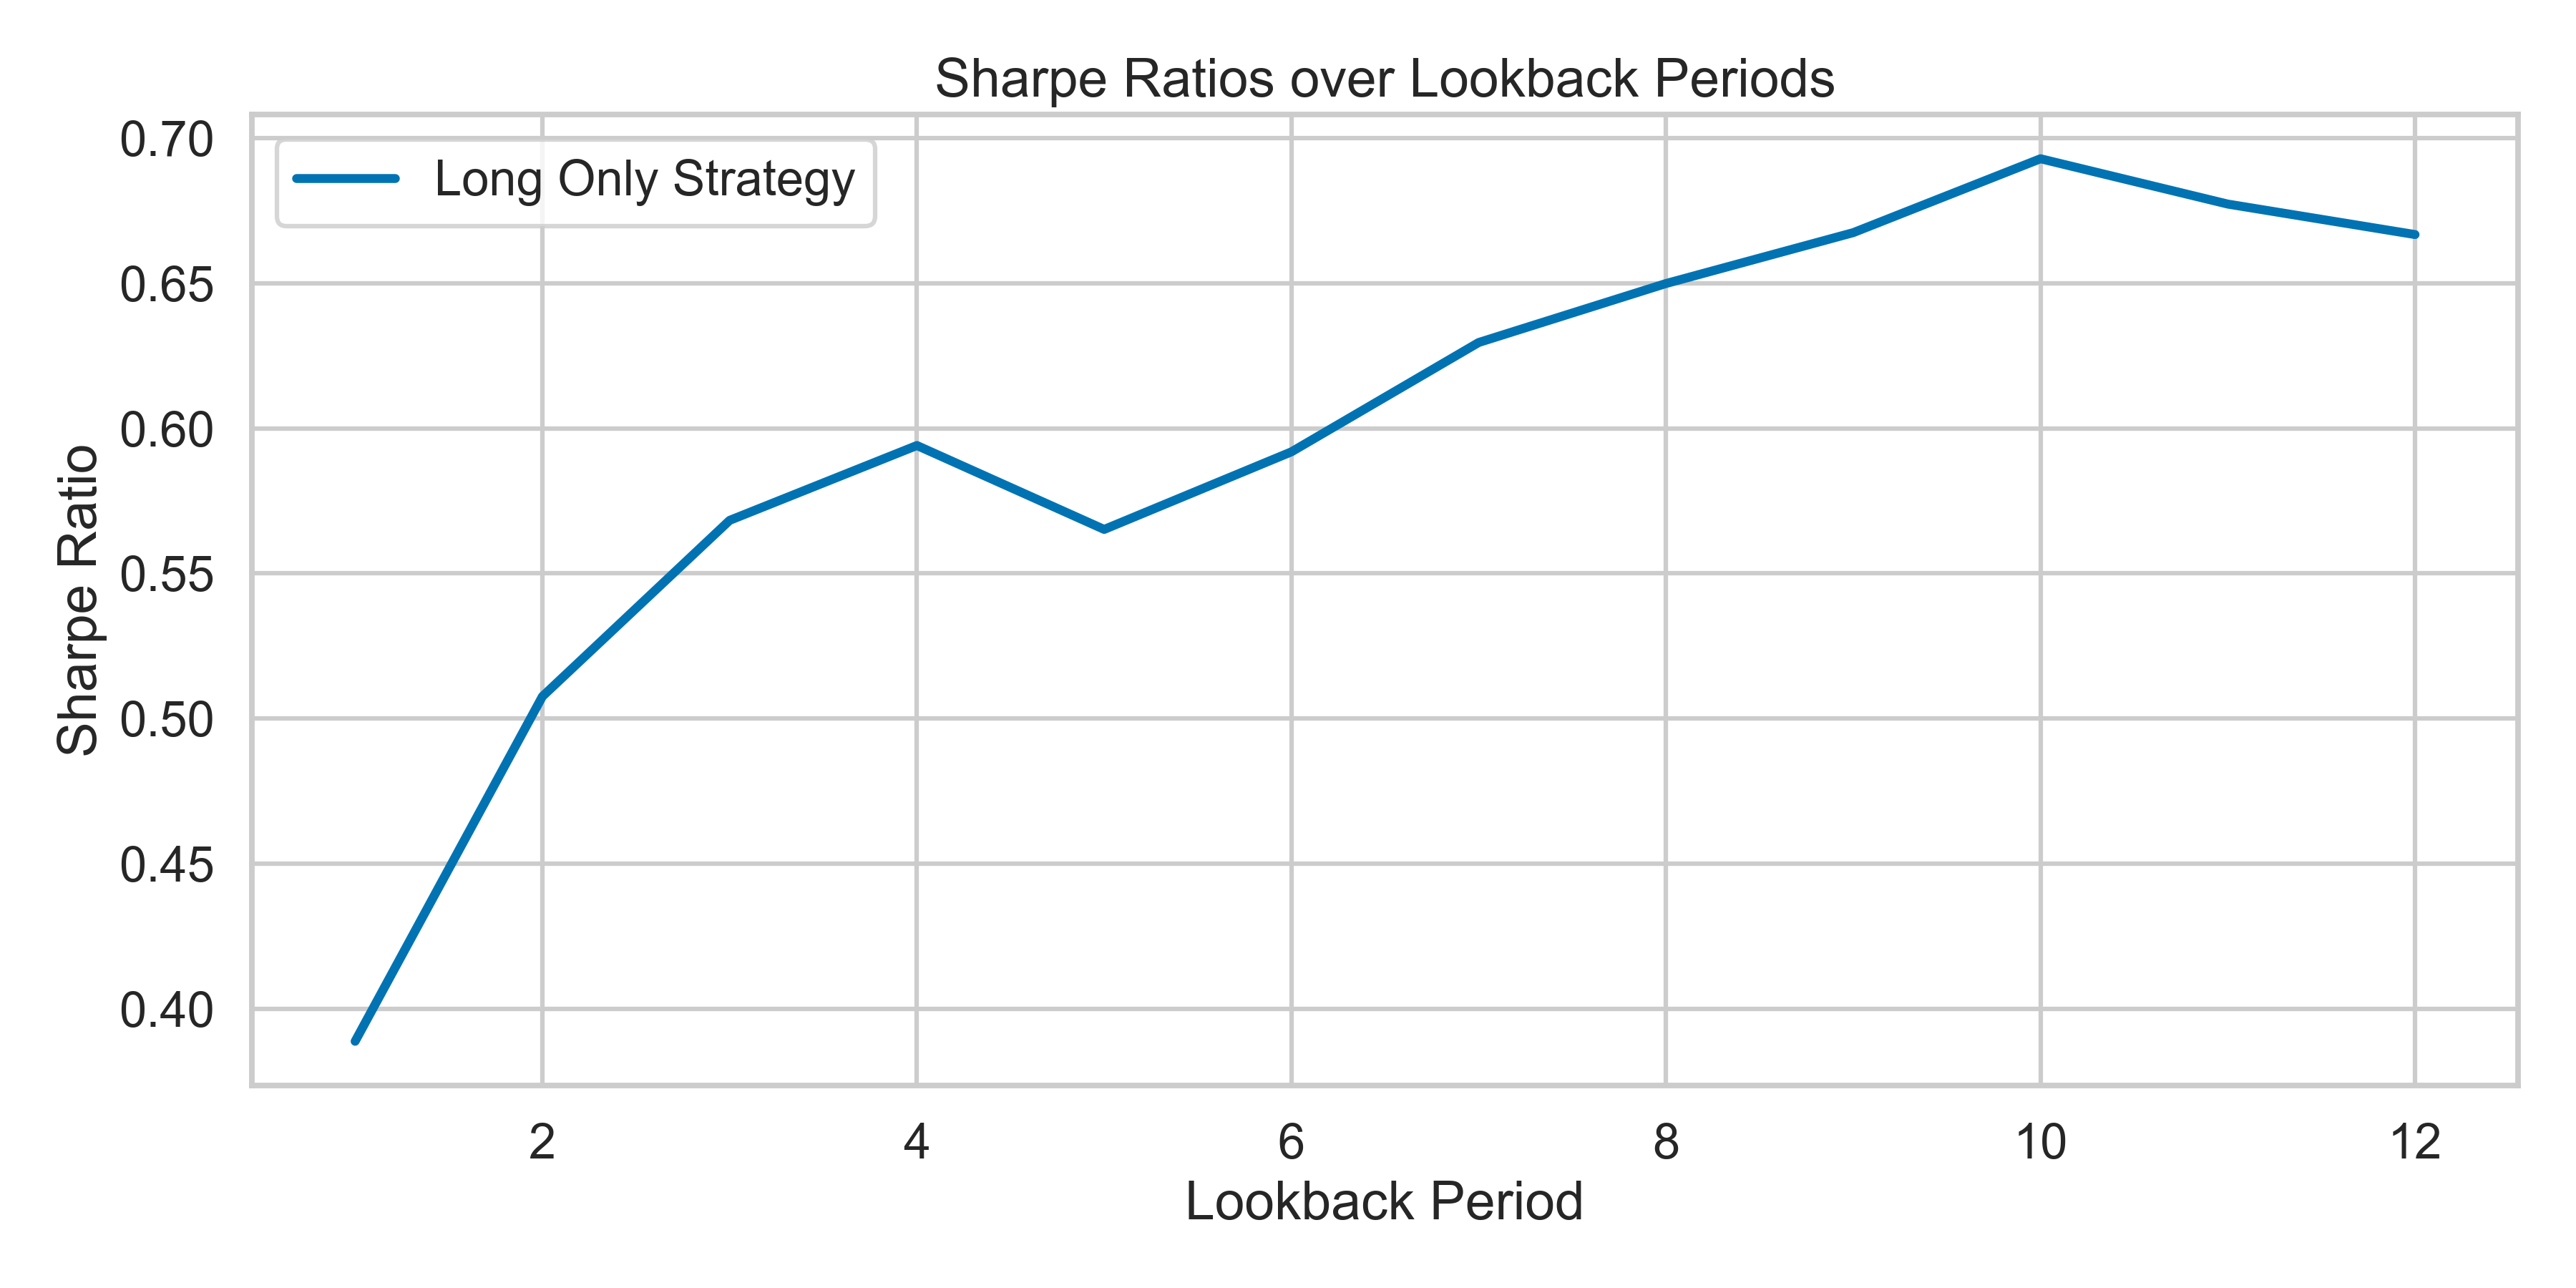
\includegraphics[width=\linewidth]{figures/rc_lookback_period.png}
    \end{figure}
\end{frame}

\begin{frame}{Robustness Check: Varying Number of Assets Held}
  \begin{figure}
   \caption{Sharpe Ratios Over Different Number of Assets Held}
        \centering
        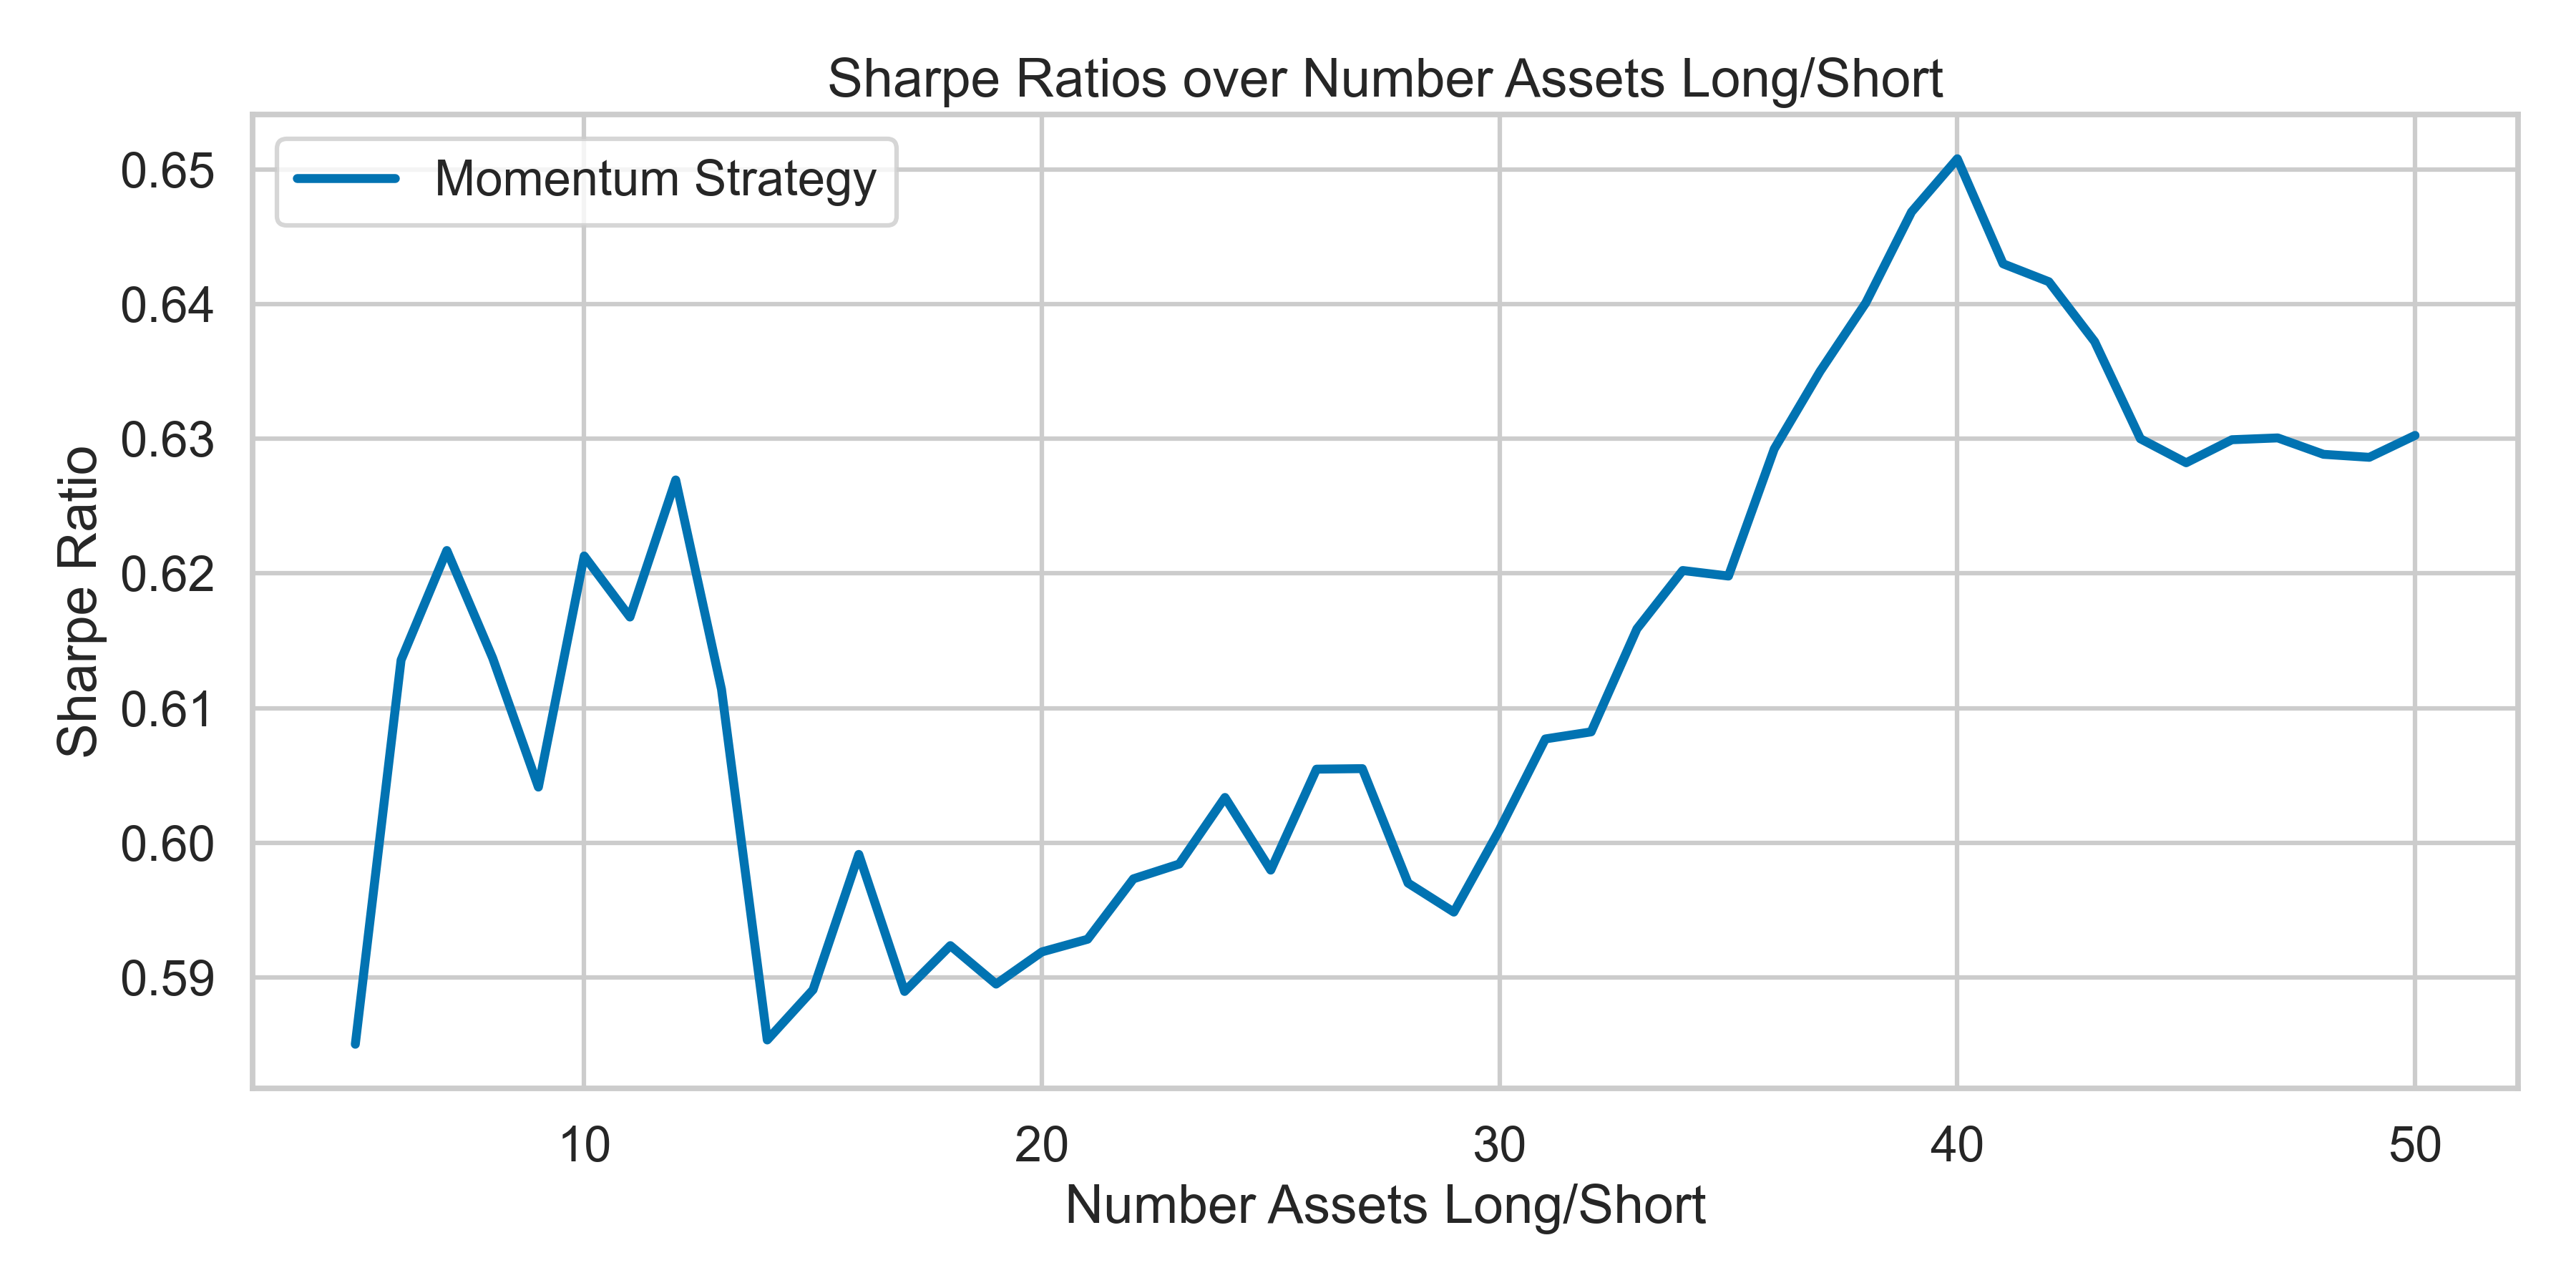
\includegraphics[width=\linewidth]{figures/rc_number_assets.png}
    \end{figure}
\end{frame}

\begin{frame}{Robustness Check: Varying Transaction Costs}
  \begin{figure}
   \caption{Net-Cumulative Total Returns: Long Only Momentum vs. SPI}
        \centering
        \includegraphics[width=\linewidth]{figures/rc_trxCost.png}
    \end{figure}
\end{frame}
=======
>>>>>>> 1a19774ded2f08b42fe103161d958e218e36807a

%Conclusion
\section{Conclusion}
\begin{frame}{Conclusion}

\begin{itemize}
    \item Long-only momentum strategy generates substantial outperformance compared to the SPI benchmark, even after accounting for transaction costs.
    \item Long-only underperformed relative to the corresponding long/short strategy.
    \item A negative relationship between holding periods and Sharpe ratios exists, suggesting shorter holding periods may be more effective.
    \item The lookback period analysis showed a peak in performance at around 10 months. 
<<<<<<< HEAD
    \item Increasing number of assets held increases Sharpe Ratio due to diversification effects, which diminish at a certain amount of assets.
    \item Resilience to transaction costs, remaining profitable even with costs up to 1\%.  
    \item In short: Momentum strategies can be profitable but careful consideration must be given to parameters such as holding period, lookback period, number of assets held and, most importantly, the investment universe. 
=======
    \item Resilience to transaction costs, remaining profitable even with costs up to 1\%.      
>>>>>>> 1a19774ded2f08b42fe103161d958e218e36807a
\end{itemize}
\end{frame}

%References
\section{References}
\begin{frame}{References}

<<<<<<< HEAD
\printbibliography


=======
\begin{itemize}
    \item Ammann, M. and M. Steiner (2008). “Risk Factors for the Swiss Stock
Market”. In: Schweizerische Zeitschrift f¨ur Volkswirtschaft und Statistik
144(1), pp. 1–35. doi: 10.1007/BF03399247.
    \item De Bondt, W. F. and R. Thaler (1987). “Further Evidence on Investor
Overreaction and Stock Market Seasonality”. In: The Journal of Finance
42(3), pp. 557–581. doi: 10.1111/j.1540-6261.1987.tb04569.x.
    \item Jegadeesh, N. and S. Titman (1993). “Returns to Buying Winners and Selling Losers: Implications for Stock Market Efficiency”. In: The Journal of Finance 48(1), pp. 65–91. doi: 10.2307/2328882.
    \item Rouwenhorst, G. K. (1998). “International Momentum Strategies”. In: The Journal of Finance 53(1), pp. 276–284. doi: 10.1111/0022-1082.95722.

    
\end{itemize}
>>>>>>> 1a19774ded2f08b42fe103161d958e218e36807a
\end{frame}

\end{document}
